\section{Hyperbolic Functions}

\begin{definition}[hyperbolic functions]
The functions \emph{hyperbolic cosine} and \emph{hyperbolic sine} are defined,
for every $x\in \RR$, as follows:
\mymargin{$\sinh$, $\cosh$}%
\index{$\sinh$, $\cosh$}%
\index{functions!hyperbolic}%
\index{sine!hyperbolic}%
\index{cosine!hyperbolic}%
\index{$\sinh$}%
\index{$\cosh$}%
\begin{equation}
\label{eq:sinh_cosh}
  \cosh x = \frac{e^x + e^{-x}}{2},
  \qquad
  \sinh x = \frac{e^x - e^{-x}}{2}.
\end{equation}
\end{definition}

\begin{theorem}[properties of hyperbolic functions]
The following properties hold.
\begin{enumerate}
\item
The function $\sinh$ is odd, $\cosh$ is even:
\[
\sinh(-x) = -\sinh(x),
\qquad
\cosh(-x) = \cosh(x);
\]

\item
The points in the plane with coordinates $(\cosh x, \sinh x)$ for $x\in \RR$ lie
on a branch of a hyperbola since the following holds:
\[
  \cosh^2 x - \sinh^2 x = 1;
\]

\item addition formulas:
\begin{align*}
  \cosh(\alpha+\beta) &= \cosh \alpha \cosh \beta + \sinh \alpha \sinh \beta,\\
  \sinh(\alpha+\beta) &= \sinh \alpha \cosh \beta + \cosh \alpha \sinh \beta;
\end{align*}

\item
The function $\sinh$ is strictly increasing on all of $\RR$, the function
$\cosh$ is strictly increasing on the interval $[0,+\infty)$ and strictly
decreasing on the interval $(-\infty,0]$;

\item as $x\to +\infty$, $\sinh x \to +\infty$, $\cosh x \to +\infty$, and as $x\to -\infty$, $\sinh x \to -\infty$, $\cosh x \to +\infty$.

\end{enumerate}
\end{theorem}

\newsavebox{\qrfigiperb}\sbox{\qrfigiperb}{\myurlhere{figiperb}{hyperbolic functions}}%
\begin{figure}
  \centering%
  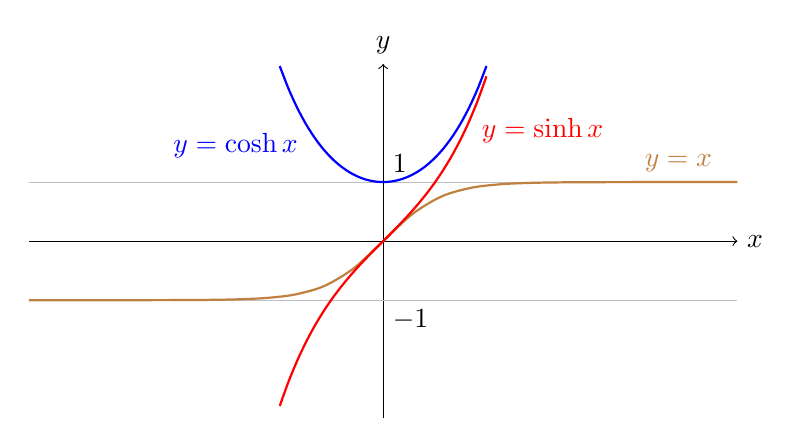
\begin{tikzpicture}[scale=0.75]
  \draw[->] (-6,0) -- (6,0) node[right] {$x$};
  \draw[->] (0,-3) -- (0,3) node[above] {$y$};
  \foreach \y in {1, -1} {
    \draw[shift={(0,\y)},lightgray] (-6,0) -- (6,0);
  }
  \draw (0,1) node [above right] {$1$};
  \draw (0,-1) node [below right] {$-1$};
  \draw[domain=-6:6,smooth,variable=\x,brown,thick] plot ({\x},{tanh(\x)});
  \draw[domain=-1.75:1.75,smooth,variable=\x,blue,thick] plot ({\x},{cosh(\x)});
  \draw[domain=-1.75:1.75,smooth,variable=\x,red,thick] plot ({\x},{sinh(\x)});
  \draw (-2.5,2) node[blue,below] {$y=\cosh x$};
  \draw (2.7,1.5)  node[red,above] {$y=\sinh x$};
  \draw (5,1) node[brown,above] {$y=\tgh x$};
  \end{tikzpicture}
  \caption{%
    The graphs of the functions $\sinh$, $\cosh$, and $\tgh$.
    \ifwidemargin\\\\\fi%
    \usebox{\qrfigiperb}%
  }
\end{figure}

\begin{proof}
The first three points can be easily proven by direct verification, using the
definition~\eqref{eq:sinh_cosh}.

Regarding monotonicity, observe that if $x\ge 0$, each term of the two series
mentioned in point 4 is strictly increasing (since all coefficients are
positive), and thus the sums of the series, i.e., the function $\cosh$ and the
function $\sinh$, are strictly increasing on the interval $[0,+\infty)$. The
function $\sinh$, being odd, is also increasing on the interval $(-\infty,0]$
and therefore is increasing on all of $\RR$.

For the last property, it suffices to use the definition~\eqref{eq:sinh_cosh}
and recall that (theorem~\ref{th:ordine_infinito}) if $x\to +\infty$, then
$e^x\to +\infty$ and $e^{-x}=\frac{1}{e^{x}} \to 0$.
\end{proof}

We observe that $\cosh 0 = 1$ and, due to the monotonicity properties seen in
the previous theorem, we have $\cosh x \ge \cosh 0 = 1 > 0$. Thus, $\cosh x$
never vanishes, and for every $x\in \RR$, the \emph{hyperbolic tangent} can be
defined
\index{tangent!hyperbolic}%
\mymargin{$\tgh$}%
\index{$\tgh$}%
\[
    \tgh x = \frac{\sinh x}{\cosh x}.
\]

The function $\sinh\colon \RR\to\RR$ is injective since it is strictly
increasing and is surjective since it is continuous and thus takes all values
between $\lim_{x\to+\infty} \sinh(x) = +\infty$ and $\lim_{x\to -\infty}
\sinh(x) = -\infty$. Therefore, $\sinh\colon \RR \to \RR$ is invertible, and the
inverse function is called the \emph{hyperbolic sine sector} and is denoted by
\mymargin{$\settsinh$}%
\index{$\settsinh$}
\index{sector!of hyperbolic sine}
\[
    \settsinh \colon \RR \to \RR.
\]
Similarly, the restricted function $\cosh\colon [0,+\infty)\to [1,+\infty)$ is
injective since it is strictly increasing and is surjective since it is
continuous and takes all values between $\cosh(0)=1$ and $\lim_{x\to +\infty}
\cosh x = +\infty$ on $[0,+\infty)$. Therefore, the function $\cosh x$
restricted to $[0,+\infty)\to [1,+\infty)$ is invertible, and the inverse
function is called the \emph{hyperbolic cosine sector}
\mymargin{$\settcosh$}%
\index{$\settcosh$}
\index{sector!of hyperbolic cosine}
\[
    \settcosh \colon [1,+\infty)\to [0,+\infty).
\]

The function $\tgh x$ is strictly increasing on all of $\RR$ and takes all
values strictly between $-1$ and $1$. The inverse function is called $\setttgh$.

\begin{exercise}
Given $y\in \RR$, solve the equation
\[
    \frac{e^x - e^{-x}}{2} = y
\]
by reducing it to a quadratic equation in the variable $t=e^x$. Then prove that
\[
    \settsinh x = \ln\enclose{x + \sqrt{x^2 + 1}}.
\]
Similarly, prove that
\[
    \settcosh x = \ln\enclose{x + \sqrt{x^2 - 1}}
\]
and
\[
    \setttgh x = \ln \sqrt{\frac{1+x}{1-x}}.
\]
\end{exercise}